\documentclass[10pt,aspectratio=169]{beamer}

% All the boilerplate is in deslides.sty
\usepackage{deslides}

\author{Ji\v{r}\'i Lebl}

\institute[OSU]{%
Oklahoma State University%
%Departemento pri Matematiko de Oklahoma {\^S}tata Universitato%
}

\title{11. Exact equations (part 1)\\(Notes on Diffy Qs, 1.8)}

\date{}

\begin{document}

\begin{frame}
\titlepage

%\bigskip

\begin{center}
The textbook: \url{https://www.jirka.org/diffyqs/}
\end{center}
\end{frame}

\begin{frame}
An \emph{exact equation} is an equation that encodes 
\[
F(x,y) = \text{constant}
\]
for a \emph{potential function} $F(x,y)$.

\medskip
\pause

Naming suggests electric potential or potential energy.

\medskip
\pause

Such equations come up when there is some conservation
law at play.

(e.g., conservation of energy)

\end{frame}

\begin{frame}
\textbf{Example:}
Let $F(x,y) = x^2+y^2$

%16 is the number of lines, must be adjusted
\vspace*{-\baselineskip}
\hspace*{3in}%
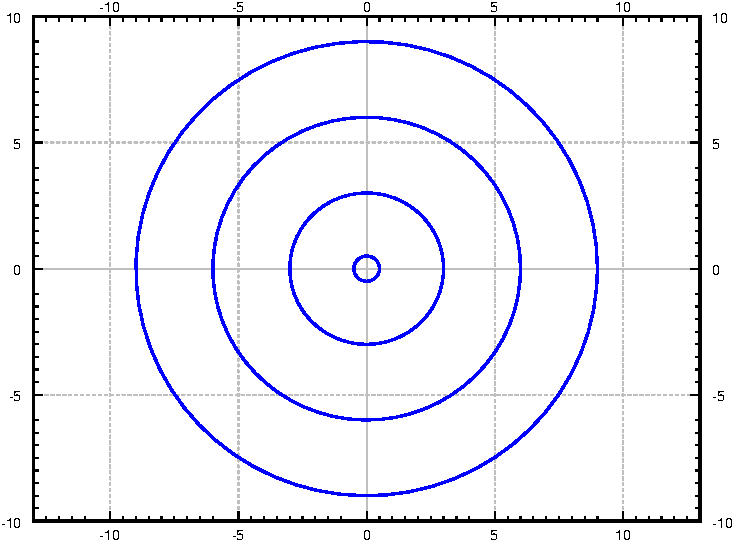
\includegraphics[width=2.5in]{../figures/circlesfig}

\hspace*{3in}%
Solutions to $F(x,y) = x^2+y^2 = C$.

\vspace*{-1.8in}

\pause

Take the
\emph{total derivative} of
$F$:

\medskip
\quad
$dF =
\dfrac{\partial F}{\partial x} dx + \dfrac{\partial F}{\partial y} dy
=
F_x dx + F_y dy
$.

\medskip
\pause
So
$dF = 2x \, dx + 2y \, dy$.

\medskip
\pause

The differential equation for
$F(x,y) = C$
is

\medskip

\quad $dF = 0$.

\medskip
\pause

In this case,

\medskip

\quad
$2x \, dx + 2y \, dy = 0$
\quad
or
\quad
$2x + 2y \, \dfrac{dy}{dx} = 0$
\end{frame}

\begin{frame}

In general, \quad
$M \, dx + N \, dy = 0$, \quad
or
\quad
$M + N \, \frac{dy}{dx} = 0$ \quad
is exact if it is \quad $dF = 0$.

\medskip
\pause

In other words, $M \, dx + N \, dy = 0$ is exact if there is an $F$ such that $M = F_x$ and $N=F_y$.

\medskip
\pause

So 
\quad
$2x \, dx + 2y \, dy = 0$
\quad
is exact.

\medskip
\pause

$x^2+y^2=C$ are implicit solutions.

\medskip
\pause

$y = \pm \sqrt{C-x^2}$ are the explicit solutions.

\medskip
\pause

Normally, we start with $M \, dx + N \, dy = 0$ and we wish to find the
unknown $F(x,y)$.
\end{frame}

\begin{frame}
\textbf{Interpretation:}
At each point $(x,y)$ there is a vector $\vec{v} = (M,N)$ giving a \emph{vector
field}.

\medskip
\pause

$\vec{v}$ is a \emph{conservative vector field} if it comes with a potential
function $F$, where
$\vec{v} = \left( \frac{\partial F}{\partial x} ,\frac{\partial F}{\partial
y} \right)$.

\medskip
\pause

Let $\gamma$ be a path in the plane from $(x_1,y_1)$ and ending at
$(x_2,y_2)$ and think of $\vec{v}$ as force.

\medskip

The work required to move along $\gamma$ is
\quad
$\displaystyle
\int_\gamma \vec{v}(\vec{r}) \cdot d\vec{r}
=
\int_\gamma M \, dx + N \, dy
=
F(x_2,y_2) - F(x_1,y_1)$.

\medskip
\pause

In other words, work done depends only on endpoints.

\medskip
\pause

\textbf{Example:} Force of gravity is conservative (assuming 2D)
--- $F$ is the gravitational potential.
\pause
Work done by moving a mass only depends on the change in elevation.

\medskip
\pause

Exact equations are conservative vector fields, and
their
implicit solutions are given by the potential functions.

\end{frame}

\begin{frame}
The process is:

\medskip

1) We are given an equation
\quad
$M + N \, \frac{dy}{dx} = 0$

\medskip
\pause

2) We determine if the equation is exact.

\medskip
\pause

3) If it is, we try to find an $F$ such that $F_x = M$
and $F_y = N$.

\medskip
\pause

$F\bigl(x,y(x)\bigr) = C$ gives an implicit solution.

\medskip
\pause

\textbf{Note:} Adding a constant to $F$ does not change anything.

\pause
If $F(x,y)$ works, $F(x,y)+3$ or $F(x,y)-8$ also work.

\end{frame}

\begin{frame}

\textbf{Example:}
Consider \quad $2x + 2y \frac{dy}{dx} = 0$. \quad  Forget we knew
what $F$ was.

\medskip
\pause

$M = 2x$ and $N=2y$.

\medskip
\pause

If $F$ exists, $F_x (x,y) = 2x$.

\medskip
\pause

Integrate in $x$:
\quad
$F(x,y) = x^2 + A(y)$,
\quad
for some function $A(y)$ (constant of integration).

\medskip
\pause

Differentiate in $y$ and set it equal to $N$:

\medskip
\quad
$2y = F_y (x,y) = A'(y)$.

\medskip
\pause

Integrate $2y=A'(y)$: \quad
$A(y) = y^2$ \quad (no need for a constant of integration).

\medskip
\pause

So

\medskip

\quad
$F(x,y) = x^2 + A(y) = x^2+y^2$.

\end{frame}

\begin{frame}

The procedure (if equation is exact):
\begin{enumerate}[(i)]
\item
\pause
Integrate $F_x = M$ in $x$ resulting in $F(x,y) = \text{something} + A(y)$.
\item
\pause
Differentiate $F$ in $y$, and set that equal to
$N$ to find $A(y)$ by integration.
\end{enumerate}
\pause
Roles of $x$ and $y$ (and so $M$ and $N$) can be reversed.

\end{frame}

\begin{frame}

\textbf{Example:}
Consider \quad $2x+y + xy \frac{dy}{dx} = 0$.

\medskip
\pause

$M = 2x+y$, \quad $N=xy$.

\medskip
\pause

We try as before.  Suppose $F$ exists.

\medskip
\pause

$F_x (x,y) = 2x+y$.

\medskip
\pause

Integrate in $x$: \quad $F(x,y) = x^2 + xy + A(y)$

\medskip
\pause

Differentiate in $y$ and set equal to $N$:

\medskip
\pause

$N = xy = F_y (x,y) = x+A'(y)$.

\medskip
\pause

But there is no way to write $xy = x+ A'(y)$, no matter what $A'(y)$ is.

\medskip
\pause

The equation is not exact!  $F$ does not exist.
\end{frame}

\begin{frame}
How to check if $F$ exists?

\medskip
\pause

If $F$ exists, then
$M = F_x$ and
$N = F_y$.

\medskip
\pause

Then
\[
\frac{\partial M}{\partial y}
\pause
=
\frac{\partial^2 F}{\partial y \partial x}
\pause
=
\frac{\partial^2 F}{\partial x \partial y}
\pause
=
\frac{\partial N}{\partial x} .
\]
\pause
In fact:

\begin{theorem}[Poincar\'e]
If $M$ and $N$ are continuously differentiable functions of $(x,y)$, and
$\frac{\partial M}{\partial y} = \frac{\partial N}{\partial x}$,
then near any point there is a function $F(x,y)$
such that
$M = \frac{\partial F}{\partial x}$ and
$N = \frac{\partial F}{\partial y}$.
\end{theorem}

\pause

\textbf{Note:} The theorem doesn't say a \emph{global} $F$ exists, only \emph{local}.

\medskip
\pause

Back to example: If $M = 2x + y$ and $N = xy$,  
then
$M_y = 1$ and  $N_x = y$.
\pause
Not equal.
\pause
Not exact.

\end{frame}

\begin{frame}

\textbf{Example:}
Solve
\quad $\displaystyle \frac{dy}{dx} = \frac{-2x-y}{x-1}$, \quad $y(0) = 1$.

\medskip
\pause

Write the equation as \quad
$\displaystyle
(2x+y) + (x-1)\frac{dy}{dx} = 0$,
\quad
\pause
so \quad $M = 2x+y$ \quad and \quad $N = x-1$.

\medskip
\pause

$M_y = 1 = N_x$
\quad
so the equation is exact.

\medskip
\pause

Integrate $M$ in $x$:
\quad
$F(x,y) = x^2+xy + A(y)$

\medskip
\pause

Differentiate in $y$ and set to $N$ to find
\quad
$x-1 = x + A'(y)$

\medskip
\pause

$A'(y) = -1$ \quad so \quad $A(y) = -y$ works.
\quad
\pause
Take \quad $F(x,y) = x^2+xy-y$.

\medskip
\pause

Implicit (general) solution is \quad
$x^2+xy-y = C$

\medskip
\pause

$y(0)=1$ \wthus $F(0,1) = C$ \pause \wthus $0^2+0\times 1 - 1 = C$ \pause
\wthus $C=-1$.

\medskip
\pause

Finally, solve $x^2+xy-y = -1$ for $y$:
\[
y = \frac{-x^2-1}{x-1} .
\]
\end{frame}

\begin{frame}

\textbf{Example:}
Solve
\quad
$\displaystyle
\frac{-y}{x^2+y^2} dx + \frac{x}{x^2+y^2} dy = 0$, \quad $y(1) = 2$.
\qquad
\pause
(Exercise: $M_y = N_x$)

\medskip
\pause

The vector field
$(M,N)$ is \textbf{not} conservative on the entire plane minus the origin.

\pause
Problem: Let $\gamma$ be a circle around the origin counterclockwise
starting and ending at $(1,0)$.
\pause
If $F$ existed we would have
(computation left to interested student)
\[
0 = F(1,0) - F(1,0) \pause = \int_\gamma F_x \, dx + F_y \, dy \pause = \int_\gamma \frac{-y}{x^2+y^2} \, dx +
\frac{x}{x^2+y^2} \, dy \pause = 2\pi 
\pause
\quad
\text{Nonsense!}
\]
\pause
There is no $F$ defined for all $(x,y) \not= (0,0)$.

\medskip
\pause

The theorem only guaranteed $F$ defined \emph{locally}.

\medskip
\pause

Suppose $x > 0$ (note the IC).

\pause
Integrate $M$ in $x$ to find
\quad $F(x,y) = \operatorname{arctan} \bigl( \nicefrac{y}{x} \bigr)$.

\pause
Implicit solution:
\quad
$\operatorname{arctan} \bigl( \nicefrac{y}{x} \bigr) = C$.

\pause
Explicit solution: \quad  $y = \tan(C) x$.

\pause
As $y(1)=2$, we get $\tan(C) = 2$,

so \quad $y=2x$ \quad is the solution (only for $x > 0$).

\vspace*{-1.65in}
\hfill
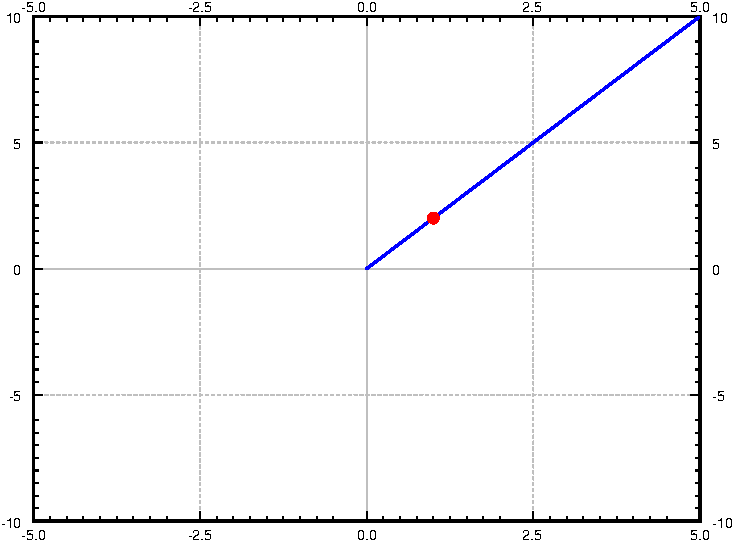
\includegraphics[width=2.5in]{../figures/exact-y2x}

\end{frame}

\end{document}
